\documentclass{article}
\usepackage{tikz}
\begin{document}
\begin{center}
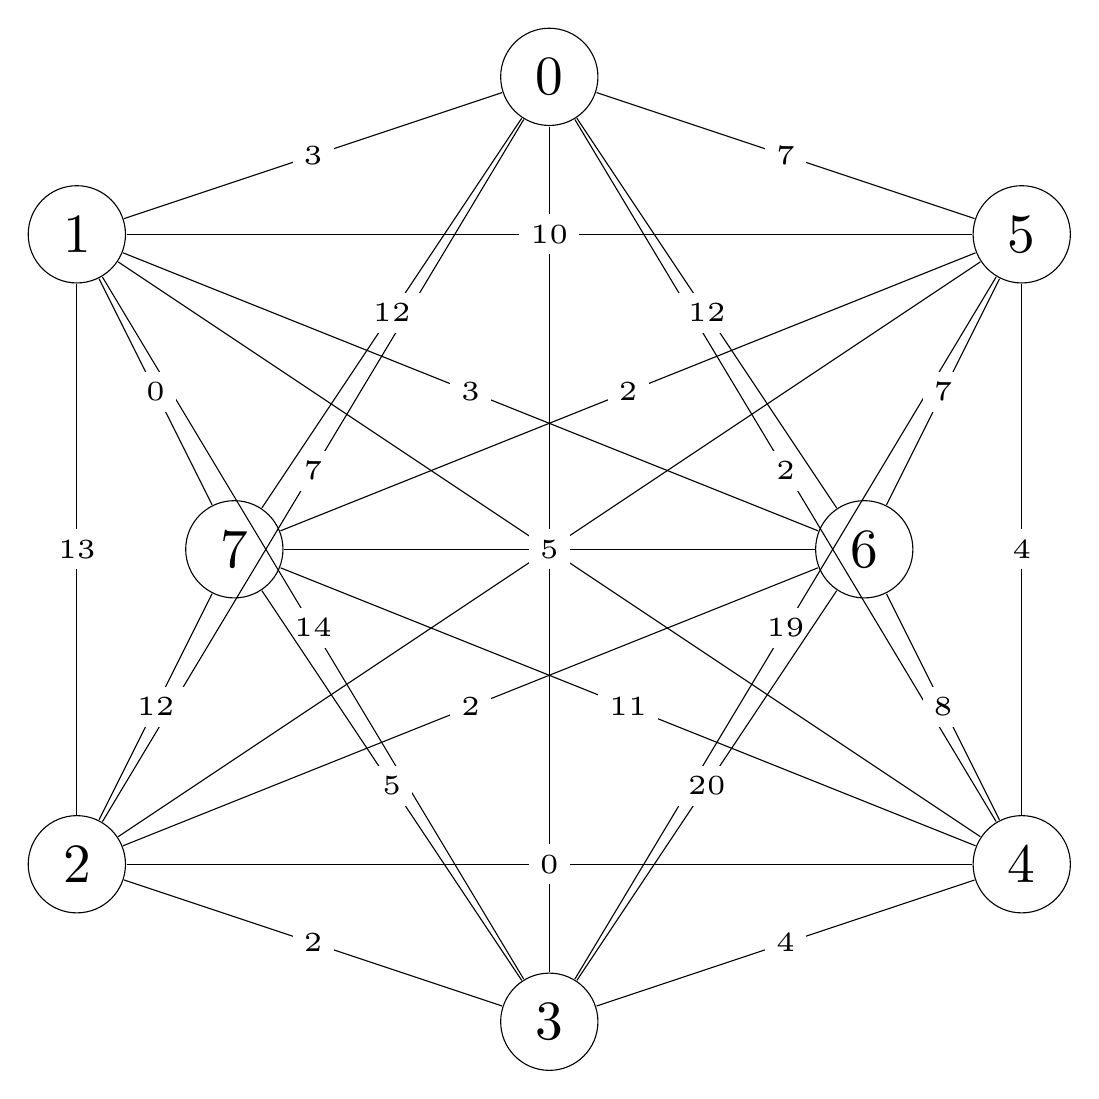
\begin{tikzpicture}[scale=2, transform shape]
% Sommets
\node[draw, circle] (0) at (0.000000, 3.000000) {0};
\node[draw, circle] (1) at (-3.000000, 2.000000) {1};
\node[draw, circle] (2) at (-3.000000, -2.000000) {2};
\node[draw, circle] (3) at (0.000000, -3.000000) {3};
\node[draw, circle] (4) at (3.000000, -2.000000) {4};
\node[draw, circle] (5) at (3.000000, 2.000000) {5};
\node[draw, circle] (6) at (2.000000, 0.000000) {6};
\node[draw, circle] (7) at (-2.000000, 0.000000) {7};
\draw (0) -- (1);
\node[fill=white, inner sep=2pt, text=black, font=\tiny] at (-1.50, 2.50) {3};
\draw (0) -- (2);
\node[fill=white, inner sep=2pt, text=black, font=\tiny] at (-1.50, 0.50) {7};
\draw (0) -- (3);
\node[fill=white, inner sep=2pt, text=black, font=\tiny] at (0.00, 0.00) {6};
\draw (0) -- (4);
\node[fill=white, inner sep=2pt, text=black, font=\tiny] at (1.50, 0.50) {2};
\draw (0) -- (5);
\node[fill=white, inner sep=2pt, text=black, font=\tiny] at (1.50, 2.50) {7};
\draw (0) -- (6);
\node[fill=white, inner sep=2pt, text=black, font=\tiny] at (1.00, 1.50) {12};
\draw (0) -- (7);
\node[fill=white, inner sep=2pt, text=black, font=\tiny] at (-1.00, 1.50) {12};
\draw (1) -- (2);
\node[fill=white, inner sep=2pt, text=black, font=\tiny] at (-3.00, 0.00) {13};
\draw (1) -- (3);
\node[fill=white, inner sep=2pt, text=black, font=\tiny] at (-1.50, -0.50) {14};
\draw (1) -- (4);
\node[fill=white, inner sep=2pt, text=black, font=\tiny] at (0.00, 0.00) {3};
\draw (1) -- (5);
\node[fill=white, inner sep=2pt, text=black, font=\tiny] at (0.00, 2.00) {10};
\draw (1) -- (6);
\node[fill=white, inner sep=2pt, text=black, font=\tiny] at (-0.50, 1.00) {3};
\draw (1) -- (7);
\node[fill=white, inner sep=2pt, text=black, font=\tiny] at (-2.50, 1.00) {0};
\draw (2) -- (3);
\node[fill=white, inner sep=2pt, text=black, font=\tiny] at (-1.50, -2.50) {2};
\draw (2) -- (4);
\node[fill=white, inner sep=2pt, text=black, font=\tiny] at (0.00, -2.00) {0};
\draw (2) -- (5);
\node[fill=white, inner sep=2pt, text=black, font=\tiny] at (0.00, 0.00) {9};
\draw (2) -- (6);
\node[fill=white, inner sep=2pt, text=black, font=\tiny] at (-0.50, -1.00) {2};
\draw (2) -- (7);
\node[fill=white, inner sep=2pt, text=black, font=\tiny] at (-2.50, -1.00) {12};
\draw (3) -- (4);
\node[fill=white, inner sep=2pt, text=black, font=\tiny] at (1.50, -2.50) {4};
\draw (3) -- (5);
\node[fill=white, inner sep=2pt, text=black, font=\tiny] at (1.50, -0.50) {19};
\draw (3) -- (6);
\node[fill=white, inner sep=2pt, text=black, font=\tiny] at (1.00, -1.50) {20};
\draw (3) -- (7);
\node[fill=white, inner sep=2pt, text=black, font=\tiny] at (-1.00, -1.50) {5};
\draw (4) -- (5);
\node[fill=white, inner sep=2pt, text=black, font=\tiny] at (3.00, 0.00) {4};
\draw (4) -- (6);
\node[fill=white, inner sep=2pt, text=black, font=\tiny] at (2.50, -1.00) {8};
\draw (4) -- (7);
\node[fill=white, inner sep=2pt, text=black, font=\tiny] at (0.50, -1.00) {11};
\draw (5) -- (6);
\node[fill=white, inner sep=2pt, text=black, font=\tiny] at (2.50, 1.00) {7};
\draw (5) -- (7);
\node[fill=white, inner sep=2pt, text=black, font=\tiny] at (0.50, 1.00) {2};
\draw (6) -- (7);
\node[fill=white, inner sep=2pt, text=black, font=\tiny] at (0.00, 0.00) {5};
\end{tikzpicture}
\end{center}
\end{document}
